\chapter{Transformaciones lineales}

Ya definimos y estudiamos el concepto de espacio vectorial, dimos
también unos ejemplos que ilustran lo útil que puede ser considerar
espacios vectoriales como marcos teóricos para modelar situaciones
prácticas. Lo que queremos hacer ahora es establecer relaciones entre
espacios vectoriales; más formalmente, queremos 
trabajar con funciones de un espacio vectorial a otro
que preserven la estructura algebráica de estos. Como veremos,
algunos de los conceptos matemáticos más usados pueden
verse de forma natural como transformaciones lineales, por ejemplo,
\begin{itemize}
	\item las operaciones de integración y diferenciación
	del cálculo, o 
	\item las proyecciones, reflexiones y proyecciones de
	la geometría.
\end{itemize}


Explicaremos además cómo codificar la información de una
transformación lineal 
entre espacios vectoriales finito
dimensionales en una matríz (que dependerá de las bases
escogidas para el dominio y codominio), hecho que hará que la teoría
desarrollada sea fácilmente llevada a la práctica - pues estaremos
sustituyendo a las funciones por objetos discretos.

\begin{figure}[H]
	\sidecaption{
	Euclides usa en sus argumentos transformaciones
	lineales como las traslaciones, rotaciones y proyecciones.
	\label{fig: eucl}
	}
	\centering
	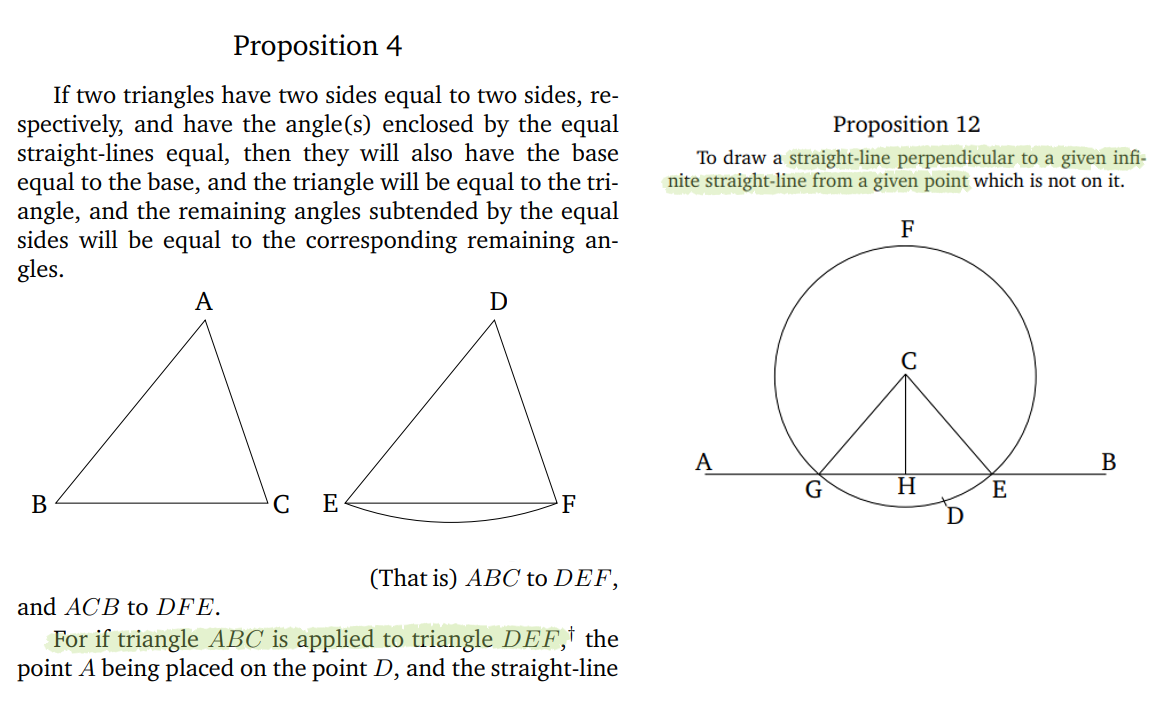
\includegraphics[scale = 2.5]{16} 
\end{figure}	

\section{Transformaciones lineales}

\begin{defi}
Sean $V$, $W$ dos espacios vectoriales sobre un mismo campo $F$.
\marginnote{Nota que $V$ y $W$ deben ser espacios vectoriales sobre un
campo común para que ambos lados de la ecuación
\ref{eq: condicion linealidad} tengan sentido.}
Toda función $T: V \longrightarrow W$ tal que
\begin{equation}
	\label{eq: condicion linealidad}
(\forall x, y \in V) (\forall a \in F): \hspace{0.2cm}
T(ax + y) = a T(x) + T(y)
\end{equation}
será llamada una \textbf{transformación lineal} de $V$ en $W$.
\end{defi}


\begin{obs}
Si $T: V \longrightarrow W$ es una transformación lineal, entonces
\begin{itemize}
	\item $T(0_{V}) = T(0_{W})$, y
	\item Para cualesquiera $n \geq 1$ entero, 
	$a_{1}, \ldots, a_{n} \in F$ y 
	$x_{1}, \ldots , x_{n} \in V$, 
	\[
	T \left( \sum_{i=1}^{n} a_{i}x_{i} \right) = 
	\sum_{i=1}^{n} a_{i}T(x_{i}).
	\]
\end{itemize}
\end{obs}
\noindent
\textbf{Demostración.}
En efecto, tenemos la siguiente ecuación en el grupo abeliano $W$
\[
T(0_{V}) = T(0_{V} + 0_{V}) = T(0_{V}) + T(0_{V}),
\]
luego, $T(0_{V}) = 0_{W}$. El segundo punto se demuestra
por inducción, usando a la condición \eqref{eq: condicion linealidad}
como base de inducción.
\QEDB
\vspace{0.2cm}

\hlgray{Ejercicio:} demuestra que la condición
\ref{eq: condicion linealidad} es equivalente a las siguientes dos
condiciones:
\begin{enumerate}
	\item (\textbf{aditividad})
	Para cualesquiera $x, y \in V: T(x+y) = T(x) + T(y)$,
	\item (\textbf{homogeneidad}) Para cualesquiera $x \in V$, $a \in F$, 
	$T(ax) = a T(x)$.
\end{enumerate}
Estas condiciones dicen que, no importa si primero
se realiza la suma o multiplicación escalar en el espacio $V$
y luego se aplica la transformación lineal, o si primero se llevan
los vectores a $W$ via $T$ y luego se efectua la suma o 
multiplicación escalar en $W$, el resultado es el mismo.

\subsection{Ejemplos de transformaciones lineales}

Tenemos la siguiente lista de ejemplos canónicos de transformaciones
lineales.
\begin{itemize}
	\item Dados $V$ y $W$ $F-$espacios vectoriales,
	las funciones $I_{V}: V \longrightarrow V$
	y $T_{0}: V \longrightarrow W$ definidas como
	\[
	\forall x \in V : \hspace{0.2cm}
	I_{V}(x) = x, \hspace{0.1cm}
	T_{0}(x) = 0_{W}
	\]
	son transformaciones lineales, llamadas respectivamente
	la \textbf{transformación identidad} y 
	la \textbf{transformación cero} en $V$.
	\item La función
	$T: P_{n}(\IR) \longrightarrow P_{n-1}(\IR)$
	definida como
	\[
	\forall f \in P_{n}(\IR) : \hspace{0.2cm}
	T(f) = f'
	\]
	es una transformación lineal.
	\item La función
	$T: \mathcal{C}(\IR) \longrightarrow \IR$
	definida como
	\[
	\forall f \in P_{n}(\IR) : \hspace{0.2cm}
	T(f) = \int_{a}^{b} f(t)dt
	\]
	es una transformación lineal.
	\item Sea $0 \leq \theta < 2 \pi$. La función
	$T_{\theta} : \IR^{2} \longrightarrow \IR^{2}$ definida como 
	\[
	\forall (a, b) \in \IR^{2} : \hspace{0.2cm}
	T_{\theta}(a, b) = (a cos(\theta) - b sen(\theta), 
	a sen(\theta) + b cos(\theta))
	\]
	es una transformación lineal llamada 
	\textbf{rotación de $\theta$ radianes}.
	\item La función $T:\IR^{2} \longrightarrow \IR^{2}$ definida como
	\[
	\forall (a, b) \in \IR^{2} : \hspace{0.2cm}
	T_{\theta}(a, b) = (a, -b)
	\]
	es llamada la \textbf{reflexión sobre el eje $x$}, y es una 
	transformación lineal tal que $T \circ T = T$.
	\item La función $T:\IR^{2} \longrightarrow \IR^{2}$ definida como
	\[
	\forall (a, b) \in \IR^{2} : \hspace{0.2cm}
	T_{\theta}(a, b) = (a, 0)
	\]
	es una transformación lineal, que llamamos \textbf{proyección
	sobre el eje-x}.
\end{itemize}


Profundicemos un poco más la definición de proyección.
Claramente, $W_{1} = \{ (a, 0): \hspace{0.2cm} a \in \IR \}$
y $W_{2} = \{ (0, b): \hspace{0.2cm} b \in \IR \}$
son subespacios de $\IR^{2}$ tales que 
$\IR^{2} = W_{1} \oplus W_{2}$. Se definió arriba a la proyección
sobre el eje-x a la función que, a cada $v \in \IR^{2}$, le 
asigna su sumando correspondiente al espacio $W_{1}$.
Definamos en general el término proyección.
\begin{defi}
	\label{def: proyeccion}
Sea $V$ un $F-$espacio vectorial, $W_{1} \leq V$.
Si $W_{2} \leq V$ es tal que $W_{1} \oplus W_{2} = V$, 
la función $T: V \longrightarrow V$ definida como
\begin{equation}
	\label{eq: proyeccion sobre W1}
	T(x) = x_{1}, \hspace{0.4cm}
x = x_{1} + x_{2}, \hspace{0.2cm}
x_{1} \in W_{1}, x_{2} \in W_{2}
\end{equation}
es llamada
una \textbf{proyección sobre $W_{1}$}.
\end{defi}

\begin{nota}
	Si $U, V, W$ son subespacios de
	un $F-$espacio vectorial, la igualdad $U \oplus V = U \oplus W$ 
	\textbf{no implica} la igualdad $V = W$.
	
	Por ejemplo, considérese a los subespacios de $\IR^{2}$
	\[
	U = span(\{(1, 0)\}), \hspace{0.2cm} \textit{ eje x},
	\]
	\[
	V = span(\{(0, 1)\}), \hspace{0.2cm} \textit{ eje y},
	\]
	\[
	W = span(\{(1, 1)\}), \hspace{0.2cm} \textit{ gráfica de la recta $y = x$}.
	\]
	Puesto que $U \cap V = \{0\} = U \cap W$, la suma de $U$ con 
	$V$ y de $U$ con $W$ es directa (c.f. Proposición
	\ref{prop: suma directa sii interseccion cero}), y de hecho es todo el espacio:
	\[
	U \oplus V = \IR^{2} = U \oplus W.
	\]
	Sin embargo, claro que $V \neq W$. 
	Observa que 
	\[
	\forall (x, y) \in \IR^{2}: \hspace{0.2cm}
	x (1, 0) + y (0, 1) = (x, y) = (x-y) (1, 0) + y(1, 1).
	\]
	$\diamond$
\end{nota}


Observe que, como se usa una suma directa para
definir una proyección, la expresión
\eqref{eq: proyeccion sobre W1}
en efecto define una función $T$, de hecho lineal, pues,
si $x = x_{1} + x_{2}$, $y = y_{1} + y_{2}$ y $a \in F$,
entonces,
\[
T(ax + y) = 
T((ax_{1} + y_{1}) + (x_{2}+y_{2}))
= ax_{1} + x_{2} =
a T(x_{1}) + T(x_{2}).
\] 
Note que $W_{1} = \{ x \in V  | \hspace{0.2cm} T(x) = x \}$,
es decir, el conjunto de puntos fijos de una proyección
en $W_{1}$ coincide con $W_{1}$. 
En la Definición \ref{def: proyeccion}
hablamos de ``una'' proyección a $W_{1}$; esto es porque, 
como mostramos a continuación, hay tantas
transformaciones lineales que satisfacen la 
definición de proyección
a $W_{1}$ como subespacios cuya suma directa
con $W_{1}$ es todo el espacio.

\begin{prop}
Sea $W_{1} \leq V$. Si $W_{2}, \tilde{W_{2}}$ son dos
subespacios de $V$ distintos entre si tales que
$V = W_{1} \oplus W_{2} = W_{1} \oplus \tilde{W_{2}}$, entonces
las transformaciones lineales
$T, \tilde{T}: V \longrightarrow V$ definidas como
\[
T(x) = x_{1}, \hspace{0.4cm}
x = x_{1} + x_{2}, \hspace{0.2cm}
x_{1} \in W_{1}, x_{2} \in W_{2}
\]
y 
\[
\tilde{T}(x) = \tilde{x}_{1}, \hspace{0.4cm}
x = \tilde{x}_{1} + 
\tilde{x}_{2}, \hspace{0.2cm}
\tilde{x}_{1} \in W_{1}, 
\tilde{x}_{2} \in \tilde{W_{2}}
\]
son distintas entre si.
\end{prop}
\noindent
\textbf{Demostración.}
Busquemos un punto en el que $T$
y $\tilde{T}$ difieren. Como 
$W_{2} \neq \tilde{W_{2}}$, sin pérdida de generalidad
podemos suponer que existe $y \in \tilde{W_{2}}-W_{2}$.
Se tiene que 
\[
x_{1} + x_{2} = y = 0 + y,
\]
con $x_{1} \in W_{1}$, $x_{2} \in W_{2}$
y $y \in \tilde{W_{2}}$. Note que $x_{1}$ no es
cero, de lo contrario, se tendría
\[
y = x_{2} \in W_{2} \hspace{0.5cm}
\lightning
\]
Así, 
\[
T(y) = x_{1} \neq 0 = \tilde{T}(y).
\]
\QEDB
\vspace{0.2cm}


\begin{figure}[H]
		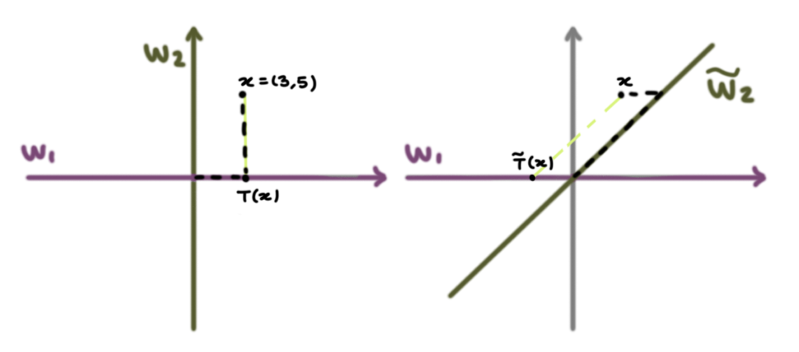
\includegraphics[scale=3.3]{17} 
 \end{figure}

\begin{ejem}
\hlpink{Poner este ejemplo mucho antes.}
Sea $V$ un $F-$espacio vectorial con $dim(V) = n$.
Si $\beta$ es una base de $V$, dividámosla en dos subconjuntos
$\alpha, \gamma$
ajenos cuya unión sea $\beta$. Entonces, $V = 
\langle \alpha \rangle \oplus \langle \gamma \rangle $,
pues 
\begin{itemize}
	\item $V = \langle \alpha \cup \gamma \rangle = 
	\langle \alpha \rangle + \langle \gamma \rangle$,
	y
	\item la suma es directa, pues
	\begin{align*}
	dim(V) = dim(\langle \alpha \rangle + \langle \gamma \rangle) &
	= dim(\langle \alpha \rangle) + 
	dim(\langle \gamma \rangle) - 
	dim(\langle \alpha \rangle \cap \langle \gamma \rangle) \\
	= & dim(V) + 
	dim(\langle \alpha \rangle \cap \langle \gamma \rangle),
	\end{align*}
	luego, $dim(\langle \alpha \rangle \cap \langle \gamma \rangle)
	= 0$, o sea, $\langle \alpha \rangle \cap \langle \gamma \rangle =
	\{ 0 \}$.
\end{itemize}
\end{ejem}
\section{El teorema fundamental de las transformaciones lineales}

La condición \eqref{eq: condicion linealidad} significa que
\marginnote{Recuerda que, si $f: A \longrightarrow B$ es una función cualquiera
y $X \subseteq A$, $Y \subseteq B$, definimos
\[
f(X) := \{ y \in B  | \hspace{0.2cm} \exists x \in X: f(x) = y \},
\]
y
\[
f^{-1}(B) = \{ x \in A  | \hspace{0.2cm} f(x) \in B \}
\]}
la función $T$ preserva la estructura algebráica de $V$. Como
veremos a continuación, toda transformación lineal también
preserva subespacios.
\begin{prop}
Sean $V$ y $W$ $F-$espacios vectoriales,
$T: V \longrightarrow W$ una transformación lineal entre estos.
\begin{itemize}
	\item La imagen de todo subespacio de $V$ bajo $T$ es un 
	subespacio de $W$, es decir,
	\[
	\forall X \subseteq V: \hspace{0.2cm}
	X \leq V \Rightarrow T(X) \leq W.
	\]
	\item La preimagen de todo subespacio de $W$ bajo $T$
	es un subespacio de $V$, es decir, 
	\[
	\forall Y \subseteq W: \hspace{0.2cm}
	Y \leq V \Rightarrow T^{-1}(Y) = 
	\{ x \in V  | \hspace{0.2cm} T(x) \in Y \} \leq V.
	\]
\end{itemize}
\end{prop}
\noindent
\textbf{Demostración.}
En efecto, si $X$ es un subespacio de $V$,
	entonces $0_{V} \in X$, luego, 
	$0_{W} = T(0_{V}) \in T(X)$. Además, si 
	$a$ es un escalar cualquiera y 
	$y_{1}, y_{2} \in T(X)$, entonces existen
	$x_{1}, x_{2} \in V$ tales que 
	$y_{i} = T(x_{i})$, con $i = 1,2$. Así,
	\[
	ay_{1} + y_{2} = a T(x_{1}) + T(x_{2})
	= T(ax_{1} + _{2})
	\]
	es elemento de $T(X)$ pues $X$, al ser subespacio
	de $V$, contiene a $ax + y$.
La demostración del segundo punto es dual.
\QEDB
\vspace{0.2cm}

Vamos ahora a asociar a una transformación
lineal dos espacios vectoriales (uno será un subespacio del
dominio, otro del codominio) de gran importancia.
\begin{defi}
\begin{marginfigure}
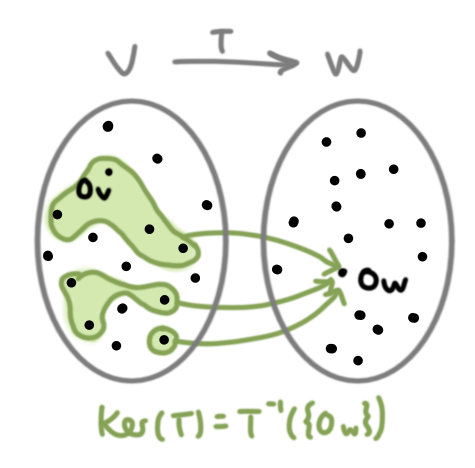
\includegraphics[scale= 2]{kernel} 
		\caption{Etimológicamente, ``kernel'' significa semilla,
		centro, esencia.}
\end{marginfigure}
Sean $V$, $W$ $F-$espacios vectoriales, $T: V \longrightarrow W$
una transformación lineal.  
\begin{itemize}
	\item Se define al \textbf{espacio nulo} de $T$
	o \textbf{kernel} de $T$ como 
	\begin{equation}
		\label{eq: kernel de T}
		Ker(T) := T^{-1}(\{ 0_{W} \}) \leq V.
	\end{equation}
	\item La \textbf{imagen} de $T$
	es \begin{equation}
		\label{eq: rango de T}
		T(V) \leq W.
	\end{equation}
\end{itemize}
\begin{marginfigure}
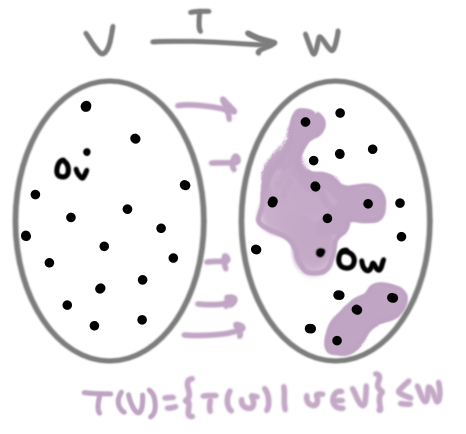
\includegraphics[scale= 2]{imagen} 
\end{marginfigure}
Si $Ker(T)$ es finito dimensional, a su dimensión se le denomina
la \textbf{nulidad de $T$}. Si $T(V)$ es finito dimensional,
su dimensión se conoce como el \textbf{rango de $T$}.
\end{defi}

Observa que el ``tamaño'' del kernel de una transformación lineal
parece ser inversamente proporcional al de la imagen de esta;
en efecto, si muchos vectores pertenecen al kernel, entonces
no habrá muchos vectores en la imagen de $T$ que no sean cero,
lo que achica a $T(V)$. El siguiente teorema, pilar del 
álgebra lineal, da forma a esta intuición.

\begin{teo}
	\label{teo: fundamental de las transf lineales}
\textbf{(fundamental de las transformaciones lineales), 
\textbf{teorema de la dimensión}}
Sean $V$, $W$ $F-$ espacios vectoriales, con $V$
finito dimensional.
Para toda
transformación lineal $T: V \longrightarrow W$,
\begin{equation}
	\label{eq: dim de V es nulidad mas rango}
	dim(V) = dim(Ker(T)) + dim(T(V)),
\end{equation}
es decir, la dimensión del espacio de origen $V$
es igual a la nulidad de $T$ más el rango de $T$.
\end{teo}
\noindent
\textbf{Demostración.}
Como $V$ es finito dimensional, el kernel de $T$ también lo es.
Sea pues $\{ n_{1}, \ldots, n_{k} \}$ una base de $Ker(T)$.
Extendamos este subconjunto l.i. de $V$ a una base de $V$;
sea $\{ v_{1}, \ldots , v_{l} \}$ tal que 
\[
\beta :=
\{ n_{1}, \ldots , n_{k} \} \cup \{ v_{1}, \ldots , v_{l} \}
\]
\marginnote{El Teorema
\ref{teo: fundamental de las transf lineales} es también
conocido como el ``Teorema de la dimensión''.}
es base de $V$. Entonces, $dim(V) = k+l$.
Afirmamos que 
$\{ T(v_{1}), \ldots, T(v_{l}) \}$
es base de la imagen $T(V)$.
\begin{itemize}
	\item Sean $a_{1}, \ldots, a_{l}$ escalares tales que
	\[
	a_{1} T(v_{1}) + \cdots + a_{l} T(v_{l}) = 0_{W}
	\]
	Supongamos que alguno de ellos no es cero; sin pérdida de
	generalidad, digamos que $a_{1} \neq 0$. Por la linealidad
	de $T$, la ecuación anterior se reescribe como
	\[
	T(a_{1}v_{1} + \cdots + a_{l}v_{l}) = 0_{W},
	\]
	es decir,
	\[
	a_{1}v_{1} + \cdots + a_{l}v_{l} \in Ker(T) =
	span(\{ n_{1}, \ldots , n_{k} \}),
	\]
	por lo tanto, 
	\[
	v_{1} \in span(\{ n_{1}, \ldots , n_{k} \}
	\cup \{ v_{2}, \ldots , v_{l} \}).
	\]
	Esto, según el Lema 
	\ref{lema: S union x es ld sii x en generado de S}, contradice
	la independencia lineal de $\beta$.
	\item Claro que $\{ T(v_{1}), \ldots, T(v_{l}) \}$
	genera a $T(V)$ pues, dado $y \in T(V)$, existe 
	$x \in V$ tal que $y = T(x)$. Como $\beta$ es base de $V$,
	existen escalares $a_{i}, b_{j}$ tales que 
	\[
	x = a_{1} n_{1} + \cdots + a_{k} n_{k} + 
	b_{1}v_{1} + \cdots b_{l}v_{l};
	\]
	evaluando ambos lados de la igualdad bajo $T$ y recordando
	que los vectores $n_{i}$ son mapeados al cero (pues 
	son elementos del kernel de $T$), concluimos que
	\[
	y = T(x) = b_{1}T(v_{1}) + \cdots + b_{l}T(v_{l}).
	\]
\end{itemize}
Así, 
\[
dim(V) = k + l = dim(Ker(V)) + dim(T(V)).
\] 
\QEDB
\vspace{0.2cm}

\hlpink{Poner una nota para que ya no confundan el rango de $T$
con el codominio de $T$.}

\begin{cor}
	\label{cor: imagen de base de V bajo lineal genera a W}
Sean $V$ y $W$ son $F-$espacios vectoriales con $V$
finito dimensional, $T: V \longrightarrow W$ lineal.
Para toda $\beta \subseteq V$ base de $V$ se tiene que
$T(\beta)$ genera a $T(V)$.
\end{cor}



\subsection{No ejemplos de transformaciones lineales}

\begin{itemize}
	\item La función $f: \IR \longrightarrow \IR$ definida como
	\[
	f(x) = e^{x}
	\]
	no es lineal, pues $f(0) \neq 0$ (de hecho, la exponencial
	es una función estríctamente positiva).
	\item La función valor absoluto $| \cdot | : \IR \longrightarrow \IR$
	no es lineal. Por ejemplo,
	\[
	|2+(-1)| = |1| = 1 \neq 3 = |2| + |-1|.
	\]
	\item El polinomio $f: \IR \longrightarrow \IR$
	definido como $f(x) = x^{2}$ no es una transformación lineal pues,
	en general, no se cumple que $(x+y)^{2}$ coincida con
	$x^{2} + y^{2}$. De hecho, lo que ocurre es 
	$(x+y)^{2} = x^{2} + 2xy + y^{2}$.
	\item Sea la función $f : \IR^{2} \longrightarrow \IR^{2}$ definida como
	\begin{align*}
	f(x, y )= \begin{cases}
	(2x, 0) & \textit{ si } y = 0 \\
	(x, y) & \textit{ si } y \neq 0.
	\end{cases}
	\end{align*}
	Es fácil comprobar que, a pesar de que $f$ es homogenea, no es
	lineal. Por ejemplo,
	\[
	f((1, 0) + (0, 1)) = f(1, 1) = (1, 1),
	\]
	pero
	\[
	f(1, 0) + f(0, 1) = (2, 0) + (0, 1) = (2, 1).
	\]
	\item La función coseno evaluada en cero vale uno, luego, 
	no es lineal.
	\item Según el Teorema \ref{teo: fundamental de las transf lineales},
	si $T: \IR \longrightarrow \IR$ es lineal, entonces
	\[
	1 = dim(Ker(T)) + dim(T(V)),
	\]
	luego, tenemos dos casos:
	\begin{enumerate}
		\item $dim(T(V)) = 1$, luego, como $T(V)$ es subespacio
		de $\IR$, con $\IR$ uno dimensional, tenemos que 
		$T(V)$ es suprayectiva.
		\item $dim(T(V)) = 0$, es decir,
		$dim(Ker(T)) = 1$. Puesto que $Ker(T) \leq \IR$
		y $dim(\IR) = 1$, se tiene que $Ker(T) = \IR$, luego,
		$T$ es la transformac
		ión lineal cero.
	\end{enumerate}
	Puesto que la función seno 
	\[
	sen(x) : \IR \longrightarrow \IR
	\]
	no es ni la función cero no suprayectiva, no puede ser lineal.
\end{itemize}


\section{Inyectividad y suprayectividad de transformaciones lineales}
Recuerda que, en general, si $f: V \longrightarrow W$ es una
función de un conjunto $V$ a otro conjunto $W$, $f$ se dice
\begin{itemize}
	\item \textbf{inyectiva} si
	\[
	\forall x, y \in V :\hspace{0.2cm}
	T(x) = T(y) \Rightarrow x = y,
	\]
	o, equivalentemente, si las imágenes de puntos
	distintos son distintas
	\item \textbf{suprayectiva} si 
	\[
	(\forall z \in W) \hspace{0.1cm}
	(\exists x \in V): \hspace{0.2cm} T(x) = z.
	\]
\end{itemize}
Resulta que, si $V$ y $W$ son 
$F-$espacios vectoriales y $T: V \longrightarrow W$ es,
no sólo una función, sino una transformación lineal entre ellos,
\marginnote{Veremos que, en el contexto de transformaciones lineales,
los conceptos de inyectividad e independencia
lineal están íntimamente ligados, así como los de 
suprayectividad y generación.}
entonces podemos encontrar equivalencias de ser inyectiva
o suprayectiva usando propiedades del Kernel y la 
preservación de la generación o inyectividad de subconjuntos de $V$.

\begin{prop}
	\label{prop: caracterizacion de inyectividad}
Sean $V$, $W$ dos $F-$espacios vectoriales. Si $T: V \longrightarrow W$
es lineal, las siguientes son equivalentes:
\begin{enumerate}
	\item $T$ es inyectiva
	\item $Ker(T) = \{ 0 \}$
	\item Si $X \subseteq V$ es linealmente independiente,
	entonces $T(X) \subseteq W$ es también linealmente independiente.
\end{enumerate}
\end{prop}
\noindent
\textbf{Demostración.}
\begin{itemize}
 	\item[$1) \Rightarrow 2)$] Si $x \in Ker(T)$ entonces,
 	por definición del kernel, $T(x) = 0$. Además,
 	como $T$ es lineal, también se tiene $T(0) = 0$, luego, como 
 	$T$ es inyectiva, tenemos que $x = 0$. Así, $Ker(T) = \{ 0 \}$.
 	\item[$2) \Rightarrow 1)$] Sean $x, y \in V$ tales que
 	$T(x) = T(y)$. Entonces, por la linealidad de $T$, 
 	$T(x-y) = T(x) - T(y) = 0 $, así, 
 	$x-y \in Ker(T) = \{ 0 \}$, es decir,
 	$x- y = 0$, o sea, $x = y$.
 	\item[$2) \Rightarrow 3)$] Sean $v_{1}, \ldots , v_{n} \in X$
 	cualesquiera; mostremos que $\{ T(v_{1}), \ldots , 
 	T(v_{n}) \}$ es linealmente independiente.
 	\marginnote{En la implicación $2) \Rightarrow 3)$, estamos mostrando
 	que un subconjunto finito arbitrario de $T(X)$ es l.i. suponiendo
 	que $X$ es l.i.. Recuerda que esto es necesario y suficiente para 
 	demostrar la independencia lineal de todo $T(X)$.}
 	Sean $a_{i} \in F$ escalares tales que
 	\[
 	a_{1} T(v_{1}) + \cdots + a_{n} T(v_{n}) = \hat{0}_{W}.
 	\]
 	Por ser $T$ lineal, podemos reescribir el lado izquierdo de la
 	igualdad anterior;
 	\[
 	T(a_{1}v_{1} + \cdots + a_{n}v_{n}) = \hat{0}_{W}.
 	\]
 	Esto muestra que 
 	$a_{1}v_{1} + \cdots + a_{n}v_{n} \in Ker(T) = \{ 0 \}$, luego,
 	\[
 	a_{1}v_{1} + \cdots + a_{n}v_{n} = 0_{V}.
 	\]
 	Como $X$ es l.i., esto implica que todos los escalares
 	$a_{i}$ son cero.
 	\item[$3) \Rightarrow 2)$] Supongamos que existe
 	$x \in Ker(T) - \{ 0 \}$. Como $x$ no es el vector cero, 
 	el singulete $\{ x \}$ es l.i. y, sin embargo, 
 	$\{ T(x) \} = \{ 0_{W} \}$ es l.d.. Esto contradice nuestra
 	hipótesis. 
\end{itemize}

\QEDB
\vspace{0.2cm}

\begin{prop}
\marginnote{Se demuestra que si $f: A \longrightarrow B$ es una función
suprayectiva, entonces, para todo $Y \subseteq B$,
se tiene $f(f^{-1}(Y))= Y$.}
Sean $V$, $W$ dos $F-$espacios vectoriales. Si $T: V \longrightarrow W$
es lineal, las siguientes son equivalentes:
\begin{enumerate}
	\item $T$ es suprayectiva
	\item Si $X \subseteq V$ genera a $V$ entonces $T(X)$
	genera a $W$.
\end{enumerate}
\end{prop}
\noindent
\textbf{Demostración.}
\begin{itemize}
	\item[$1) \Rightarrow 2)$] Sea $X$ un generador de $V$,
	es decir, un subconjunto tal que $span(X) = V$.
	Esto significa que el único subespacio de $V$ que contiene a 
	$X$ es el mismo $V$. Puesto que
	$X \subseteq T^{-1}(span(T(X)))$
	(pues, dado $x \in X$, $T(x) \in T(X) \subseteq 
	span(T(X))$), se tiene entonces
	$T^{-1}( span(T(X)) ) = V$. Evaluando ambos lados
	de la igualdad bajo la función suprayectiva $T$ concluimos que
	\[
	W = T(V) = T(T^{-1}( span(T(X))  )) =  span(T(X)),
	\]
	o sea, que $T(X)$ genera a $W$.
	\item[$2) \Rightarrow 1)$] V trivialmente se genera a sí mismo,
	luego, por hipótesis debe ocurrir que $T(V)$ genere a $W$, o sea,
	que 
	\[
	W = span(T(V)) = T(V),
	\]
	por lo tanto $T$ es suprayectiva.
\end{itemize}

\QEDB
\vspace{0.2cm}

\begin{prop}
Sean $V$ y $W$ dos $F-$espacios vectoriales finito dimensionales.
\begin{itemize}
	\item Si $dim(V) > dim(W)$, entonces no existen transformaciones
	lineales de $V$ en $W$ inyectivas.
	\item Si $dim(V) < dim(W)$, entonces no existen transformaciones
	lineales de $V$ en $W$ suprayectivas.
\end{itemize}
\end{prop}
\noindent
\textbf{Demostración.}
En efecto, 
\begin{itemize}
	\item si existe $T: V \longrightarrow W$ inyectiva, entonces,
	según la proposición \ref{prop: caracterizacion de inyectividad},
	$Ker(T) = \{ 0 \}$, luego, la ecuación
	\eqref{eq: dim de V es nulidad mas rango} se reescribe como
	\[
	dim(V) = dim(T(V)) \leq dim(W).
	\]
	\item Si existe $T: V \longrightarrow W$ suprayectiva,
	entonces $T(V)= W$, luego, 
	\eqref{eq: dim de V es nulidad mas rango} se reescribe como
	\[
	dim(V) = dim(Ker(T)) + dim(W) \geq dim(W).
	\]
\end{itemize}
\QEDB
\vspace{0.2cm}

\section{Isomorfismos}

\begin{defi}
\marginnote{Es decir, una transformación lineal
$T: V \longrightarrow W$ es un isomorfismo si 
$Ker(T) = \{ 0_{V} \}$ y $T(V) = W$.}
Sean $V, W$ dos $F-$espacios vectoriales. Toda transformación
lineal $T: V \longrightarrow W$ que sea biyectiva 
(i.e. inyectiva y suprayectiva) será llamada
un \textbf{isomorfismo}. Si existe un isomorfismo
entre dos espacios vectoriales $V$ y $W$
decimos que $V$ y $W$ son \textbf{isomorfos}.
\end{defi}

Recuerda de tus cursos anteriores que una \textit{función}
$f: A \longrightarrow B$ es biyectiva si y sólo si 
es invertible (i.e. si y sólo si existe una función
$g: B \longrightarrow A $ tal que $f \circ g = Id_{B}$ y
$g \circ f = Id_{A}$). Entonces, una transformación lineal
$T:V \longrightarrow W$ es un isomorfismo si y sólo si 
existe una función $U: W \longrightarrow V$ que sea su inversa.
Claro que tal inversa de existir es única, y se le suele denotar
por $T^{-1}$.
Como establecemos
a continuación, tal función es, al igual que $T$, una transformación lineal.
\begin{prop}
	Si $T: V \longrightarrow W$ es un isomorfismo, entonces
	su función inversa $T^{-1}$ es también un isomorfismo.
\end{prop}
\noindent
\textbf{Demostración.}
Basta probar la linealidad de $T^{-1}$. Sean pues
$y, z \in W$, $\lambda \in F$. Puesto que $T$ es lineal
y $u := T^{-1}(y)$, $v := T^{-1}(z)$ son vectores de $V$,
se tiene que 
\[
T( \lambda u + v) = \lambda T(u) + T(v) = \lambda y +z,
\]
luego,
\[
T^{-1}(\lambda y + z) = \lambda u + v = \lambda T^{-1}(y) + T^{-1}(z).
\]

\QEDB
\vspace{0.2cm}



Mostremos ahora que,
si $V$ es finito dimensional, entonces puede
establecerse un isomorfismo entre $V$
y otro $F-$espacio vectorial $W$ sólo si
$W$ tiene la misma dimensión que $V$.

\begin{prop}
	\label{prop: isomorfo implica misma dimension}
Sea $T: V \longrightarrow W$ lineal, con $V$
de dimensión finita. Si $T$ es un isomorfismo, entonces
$W$ también es finito dimensional y, de hecho,
$dim(W) = dim(V)$.
\end{prop}
\noindent
\textbf{Demostración.}
Digamos que $dim(V)=n$.
Por ser $T$ un isomorfismo, se tiene que
\[
Ker(T) = \{ 0_{V} \} \hspace{0.2cm} \textit{ y }
\hspace{0.2cm} T(V) = W.
\]
Además, como $V$ es finito dimensional, podemos usar el Teorema
\ref{teo: fundamental de las transf lineales}
para deducir que
\begin{align*}
n = dim(V) = & dim(Ker(T)) + dim(T(V)) \\
= & dim(\{ 0_{V} \}) + dim(W) \\
= & 0 + dim(W) = dim(W).
\end{align*} 
\QEDB
\vspace{0.2cm}
 
 
 Mostremos ahora que, cuando se trata con espacios vectoriales finito
 dimensionales, los conceptos de inyectividad, suprayectividad
 y biyectividad en transformaciones lineales son equivalentes.
\begin{teo}
	\label{teo: inyectiva sii supra sii biyect en dim finita}
Sean $V$, $W$ dos $F-$espacios vectoriales, ambos de dimensión
$n$. Entonces, para cualquier transformación lineal
$T: V \longrightarrow W$, son equivalentes
\begin{enumerate}
	\item $T$ es inyectiva
	\item $T$ es suprayectiva
	\item $T$ es biyectiva (i.e. un isomorfismo).
\end{enumerate}
\end{teo}
\noindent
\textbf{Demostración.}
Basta demostrar que $1)$ implica $2)$ y que
$2)$ implica $3)$.
\begin{itemize}
	\item[$1) \Rightarrow 2)$] Si $T$ es inyectiva entonces
	$Ker(T) = \{ 0 \}$, luego, por el Teorema 
	\ref{teo: fundamental de las transf lineales},
	\[
	n = dim(V) = dim(Ker(T)) + dim(T(V)) = 0 + dim(T(V)) =
	dim(T(V)),
	\]
	luego, como $dim(W) = n$ y $T(V) \leq W$ tiene dimensión $n$,
	concluimos que $T(V) = W$, o sea, que $T$ es suprayectiva.
	\item[$2) \Rightarrow 3)$] Si $T(V) = W$, entonces
	\[
	n = dim(Ker(T)) + dim(T(V)) = dim(Ker(T)) + dim(W)
	= dim(Ker(T)) + n,
	\]
	luego, $dim(Ker(T)) = 0$ o, equivalentemente, 
	$Ker(T) = \{ 0_{V} \}$, i.e. $T$ es inyectiva.
\end{itemize}
\QEDB
\vspace{0.2cm}

\begin{ejem}
	(para mostrar la importancia de la hipótesis de dimensión finita
	en el Teorema \ref{teo: inyectiva sii supra sii biyect en dim finita})
	Considere al $\IR-$espacio vectorial $\IR^{\IN}$ de sucesiones en $\IR$
	(c.f. Sección \ref{subs: F ev de funciones de X en F}).
	Sean $L, R : \IR^{\IN} \longrightarrow \IR^{\IN}$ las funciones definidas como
	\marginnote{A las transformaciones 
	\eqref{eq: funciones left y right shift} se les conoce como
	``right shift'' y ``left shift'', resp.}
	\begin{equation}
		\label{eq: funciones left y right shift}
		\forall x = (x_{1}, x_{2}, x_{3}, \ldots) \in \IR^{\IN}:
		\hspace{0.4cm}
		R(x) = (0, x_{1}, x_{2}, \ldots),
		\hspace{0.2cm}
		L(x) = (x_{2}, x_{3}, \ldots).
	\end{equation}
	Claro que $R$ y $L$ son ambas lineales, y que
	$L \circ R = Id_{\IR^{\IN}}$, luego, si $R$ tiene inversa,
	tiene que ser $L$. Sin embargo, 
	$R \circ L \neq Id_{\IR^{\IN}}$, por lo tanto, $R$ no es invertible,
	luego, no es un isomorfismo. Sin embargo, sí es inyectiva. Similarmente
	puede notar que $L$ no es un isomorfismo, pero que sí es
	suprayectiva. $\diamond$
\end{ejem}

\begin{ejem}	
Sea la función $T: P_{2}(\IR) \longrightarrow P_{3}(\IR)$
definida como
\[
T(f)(u) = 2 f'(u) + \int_{0}^{u} 3f(x) dx.
\hspace{0.2cm} \textit{(polinomio en la variable )} u. 
\]
Puesto que $T$ es combinación lineal de transformaciones lineales,
es también lineal. Según el Corolario 
\ref{cor: imagen de base de V bajo lineal genera a W},
$\{ T(1), T(x), T(x^{2}) \}$ genera al rango de $T$. Se calcula que
\[
T(1)(u) = 2 \cdot 0 + \int_{0}^{u} 3 dx = 3u,
\]
\[
T(x)(u) = 2 + \int_{0}^{u} 3x dx = 2 + \frac{3}{2}x^{2} \Bigg|_{x=0}^{x=u}
= 2 + \frac{3u^{2}}{2},
\]
\[
T(x^{2})(u) = 4u + \int_{0}^{u} 3x^{2}dx = 
4u + x^{3} \Bigg|_{x=0}^{x=u} = 4u + u^{3}.
\]
Tenemos entonces que 
\[
\{ g_{1}(u) = 3u, g_{2}(u) = 2 + (3/2)u^{2}, g_{3}(u) = 4u + u^{3}  \}
\]
genera a $T(P_{2}(\IR))$; puesto que los elementos de este generador
son polinomios de grados distintos, de hecho son linealmente independientes,
luego, esta es una base del rango de $T$. Así, como
$dim(P_{2}(\IR)) = 3$, se debe tener que $T$ es inyectiva.
$\diamond$
\end{ejem}

\section{La propiedad universal de las bases}
Recuerda que, dados $V$ y $W$ dos $F-$ espacios vectoriales,
una transformación lineal $T:V \longrightarrow W$
es una función que además ``abre'' combinaciones lineales. Como cualquier
función, $T$ está completamente determinada por los valores que
toma en su dominio $V$. Como veremos a continuación, 
en el caso de las transformaciones lineales, estas de hecho quedan
determinadas por su definición en una base cualquiera
del espacio $V$; conocer los valores de $T$ en una base
de $V$ nos permite saber los valores de $T$ en \textit{cualquier}
punto de $V$.
\marginnote{Al Teorema 
\ref{teo: propiedad univ de las bases} también se le conoce como el 
Teorema fundamental de las bases. Se usará en repetidas ocasiones
para desarrollar la teoría de las siguientes secciones, por lo que
se recomienda entenderlo bien.}
\begin{teo}
	\label{teo: propiedad univ de las bases}
(propiedad universal de las bases) Sea
$V$ un $F-$ espacio vectorial, con 
$V$ finito-dimensional. Son equivalentes
para $\beta \subseteq V$ las siguientes:
\begin{center}
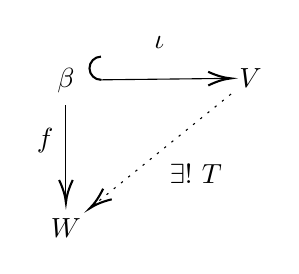
\begin{tikzpicture}[x=0.75pt,y=0.75pt,yscale=-1,xscale=1]
%uncomment if require: \path (0,235); %set diagram left start at 0, and has height of 235


% Text Node
\draw (228,104) node    {$\beta $};
% Text Node
\draw (317,103) node    {$V$};
% Text Node
\draw (228,175) node    {$W$};
% Text Node
\draw (218,133) node    {$f$};
% Text Node
\draw (288,149) node    {$^{\ } \exists !\ T$};
% Text Node
\draw (273,86) node    {$\iota $};
% Connection
\draw    (245,103.81) -- (305.5,103.13) ;
\draw [shift={(307.5,103.11)}, rotate = 179.36] [color={rgb, 255:red, 0; green, 0; blue, 0 }  ][line width=0.75]    (10.93,-3.29) .. controls (6.95,-1.4) and (3.31,-0.3) .. (0,0) .. controls (3.31,0.3) and (6.95,1.4) .. (10.93,3.29)   ;
\draw [shift={(245,103.81)}, rotate = 359.36] [color={rgb, 255:red, 0; green, 0; blue, 0 }  ][line width=0.75]      (0,-11.18) .. controls (-3.09,-11.18) and (-5.59,-8.68) .. (-5.59,-5.59) .. controls (-5.59,-2.5) and (-3.09,0) .. (0,0) ;
% Connection
\draw  [dash pattern={on 0.84pt off 2.51pt}]  (307.5,110.69) -- (241.05,164.44) ;
\draw [shift={(239.5,165.7)}, rotate = 321.03] [color={rgb, 255:red, 0; green, 0; blue, 0 }  ][line width=0.75]    (10.93,-3.29) .. controls (6.95,-1.4) and (3.31,-0.3) .. (0,0) .. controls (3.31,0.3) and (6.95,1.4) .. (10.93,3.29)   ;
% Connection
\draw    (228,116) -- (228,161) ;
\draw [shift={(228,163)}, rotate = 270] [color={rgb, 255:red, 0; green, 0; blue, 0 }  ][line width=0.75]    (10.93,-3.29) .. controls (6.95,-1.4) and (3.31,-0.3) .. (0,0) .. controls (3.31,0.3) and (6.95,1.4) .. (10.93,3.29)   ;

\end{tikzpicture}
\end{center}
\begin{itemize}
	\item $\beta$ es base de $V$
	\item Si $W$ es un $F-$espacio vectorial cualquiera, 
	toda función $f: \beta \longrightarrow W$ se puede extender
	linealmente de forma única a todo $V$, es decir, existe
	una única transformación lineal $T: V \longrightarrow W$
	tal que $T_{| \beta} = f$.
\end{itemize}
\end{teo}
\textbf{Nota:} en realidad, este teorema es cierto aún cuando
$V$ es infinito dimensional (c.f. \cite{Hugo} p. 84). Sin embargo,
como en el curso no hemos demostrado los resultados necesarios
para probar esto cuando se trabaja en un espacio infinito dimensional
(no estudiamos el Lema de Zorn, por lo que no pudimos demostrar
hechos fundamentales como la existencia de bases para cualquier
espacio vectorial o el hecho de que un l.i. de un espacio ininito
dimensional puede extenderse a una base de este), nos limitaremos
a establecer y probar la propiedad universal de las bases
en dimensión finita - que en realidad son los tipos de espacios
que se usan siempre en las aplicaciones.

\noindent
\textbf{Demostración.}
\begin{itemize}
	\item[$\Rightarrow )$] 
	Sea $f: \beta \longrightarrow W$ una función de la base
	$\beta = \{ v_{1}, \ldots , v_{n} \}$ 
	de $V$ escogida a $W$. Sean $x, y \in V$ cualesquiera;
	digamos que
	\begin{equation}
		\label{eq0: 25 sept}
		x = \sum_{i = 1}^{n} a_{i}v_{i}, \hspace{0.2cm}
		y = \sum_{i = 1}^{n} b_{i}v.
	\end{equation}
	Observe que, si $T: V \longrightarrow W$
	es una transformación lineal que extiende a $f$ (i.e.
	tal que $T \circ \iota = f$), entonces, deberá ocurrir
	\[
	T(x) = T \left( \sum_{i=1}^{n}a_{i}v_{i} \right)
	= \sum_{i=1}^{n} a_{i} T(v_{i})
	= \sum_{i=1}^{n} a_{i} \beta(v_{i}),
	\]
	es decir, $T$ \textit{tiene que ser} la función definida como
	\marginnote{Observe que la ecuación 
	\eqref{eq: definicion extension lineal de definicion en base} en efecto
	define una función $T$ de $V$ en $W$, pues, por ser $\beta$
	base de $V$, 
	la representación de $x$
	dada en \eqref{eq0: 25 sept} como combinaciones lineales de
	elementos de $\beta$ son únicas}
	\begin{equation}
		\label{eq: definicion extension lineal de definicion en base}
		T \left( \sum_{i=1}^{n}a_{i}v_{i} \right) := 
	\sum_{i=1}^{n} a_{i} \beta(v_{i}).
	\end{equation}
	Esta es en efecto una transformación lineal, pues
	\begin{align*}
	T(ax + y) = & T \left(a \sum_{i=1}^{n}a_{i}v_{i} +
	\sum_{i=1}^{n}b_{i}v_{i}\right) = T  
	\left(\sum_{i=1}^{n}(aa_{i} + b_{i} )v_{i} \right) \\
	= & \sum_{i=1}^{n} (aa_{i} + b_{i}) \beta(v_{i})
	= a\sum_{i=1}^{n} a_{i}\beta(v_{i}) + 
	\sum_{i=1}^{n} b_{i}\beta(v_{i}) = a T(x) + T(y),
	\end{align*}
	y, en efecto, $T \circ \iota = f$, pues, dado 
	$v_{i} \in \beta$ cualquiera,
	\[
	(T \circ \iota)(v_{i}) = T(v_{i}) =
	T (0v_{1} + \cdots + 1 v_{i} + \cdots + 0v_{n}) = f(v_{i}).
	\]
	\item[$\Leftarrow )$] 
	Mostremos que un subconjunto 
	$\beta = \{ v_{1}, \ldots , v_{n} \}$ de $V$ con tal propiedad
	es base de $V$.
	\begin{itemize}
		\item Independencia lineal: Supongamos que $v_{1} \in 
		\langle \beta - \{ v_{1} \} \rangle$, o sea, que existen
		escalares $c_{i}$ tales que 
		$v_{1} = \sum_{i=2}^{n}c_{i}v_{i}$. Sea la función
		$f: \beta \longrightarrow F$ definida como
		\[
		f(v_{1}) = 1, 
		\hspace{0.4cm} f(v_{i}) = 0,
		\hspace{0.2cm} 2 \leq i \leq n. 
		\]
		Sea $T$ la única extensión lineal de esta función.
		Se tiene que
		\[
		1 = T(v_{1}) = T \left( \sum_{i=2}^{n}c_{i}v_{i} \right)
		= \sum_{i=2}^{n} c_{i} T(v_{i}) = 
		\sum_{i=2}^{n} c_{i} 0_{W} = 0
		\hspace{0.2cm} \lightning 
		\]
		\item Generación: 
		Supongamos que $\beta$ no genera a $V$. Como 
		ya mostramos que $\beta$ es l.i., podemos extender $\beta$
		a una base de $V$ (c.f. corolario
		\ref{cor: extendiendo l.i. a base finita}).
		Sea pues $\gamma \subseteq V$ tal que 
		$\beta \cup \gamma$ es base de $V$. Si $f: \beta \longrightarrow V$
		se define como $f(v_{i}) = v_{i}$, observe que
		la función identidad $I_{V}: V \longrightarrow V$
		es tal que $I_{V} \circ \iota = f$, pero también la 
		proyección $T: V
		= \langle \beta \rangle
		\oplus \langle \gamma \rangle \longrightarrow V$ 
		definida como
		\[
		T(x) = b, \hspace{0.2cm} x = b + c, b \in \beta,
		c \in \gamma
		\]
		satisface que $T \circ \iota = f$. Como
		$T \neq I_{V}$, esto contradice la unicidad
		de la extensión lineal que suponemos por hipótesis.
	\end{itemize}
\end{itemize}

\QEDB
\vspace{0.2cm}

\marginnote{Es decir, para demostrar la igualdad entre transformaciones
lineales basta comprobar que sus definiciones en una base cualquiera
del dominio coinciden.}
\begin{cor}
	\label{cor: del teor fund bases}
Sea $V$, $W$ $F-$espacios vectoriales, con $V$ finito dimensional,
$T: V \longrightarrow W$, $U: V \longrightarrow W$ dos
transformaciones lineales. Si para una base
$\beta = \{ v_{1}, \ldots, v_{n} \}$ de $V$ se tiene que
\[
T(v_{i}) = U(v_{i}), \hspace{0.2cm} 1 \leq i \leq n,
\]
entonces $T = U$.
\end{cor}

Terminemos mostrando que todo $F-$espacio vectorial de 
dimensión $n$ es esencialmente $\IR^{n}$.

\begin{prop}
	\label{prop: dim V n sii V isomorfo a Rn}
Sea $V$ un $F-$ espacio vectorial. $V$ es $n-$dimensional
si y sólo si $V$ es isomorfo a $\IR^{n}$.
\end{prop}
\noindent
\textbf{Demostración.}
\begin{itemize}
	\item[$\Leftarrow$)] Inmediata de notar que $dim(\IR^{n}) = n$
	y la Proposición \ref{prop: isomorfo implica misma dimension}.
	\item[$\Rightarrow$)] Sea $\beta = \{ v_{1}, \ldots , v_{n} \}$
	base de $V$. Sea $f: \beta \longrightarrow \IR^{n}$ la función
	que a $v_{i}$ le asigna $\hat{e}_{i}$. Según la propiedad 
	universal de las bases (c.f. Teorema 
	\ref{teo: propiedad univ de las bases}), podemos extender
	a $\beta$ linealmente. Sea $T: V \longrightarrow \IR^{n}$ 
	tal extensión lineal. Puesto que $T(V)$ contiene a la 
	base canónica de $\IR^{n}$, $T(V) = \IR^{n}$, o sea,
	$T$ es suprayectiva. De esto, según el Teorema 
	\ref{teo: inyectiva sii supra sii biyect en dim finita}, se
	deduce que $T$ es un isomorfismo.
\end{itemize}
\QEDB
\vspace{0.2cm}

\section{Caracterización de transformaciones lineales de $\IR^{n}$ en $\IR^{m}$}
Es gracias a la propiedad universal de las bases establecida
en el Teorema \ref{teo: propiedad univ de las bases}
que vamos a poder caracterizar a las transformaciones lineales
entre $F-$espacios vectoriales finito
dimensionales. Como veremos más adelante, esto nos permitirá 
capturar toda la información de una transformación lineal a partir
de una cantidad finita de números, que almacenaremos en un arreglo
numérico rectangular - i.e. en una matriz.
Antes de abordar la teoría en general, para familiarizarnos
con las ideas que vamos a encontrar más adelante, estudiemos 
el caso de transformaciones lineales de un $\IR^{n}$
a un $\IR^{m}$, con $m, n \geq 1$ enteros.


Para simplificar la notación, conviene introducir la noción del
producto 
punto euclídeo en $\IR^{n}$.
\begin{defi}
Para $\hat{x} = (a_{i})_{i=1}^{n}, 
\hat{y} = (b_{i})_{i=1}^{n} \in \IR^{n}$, definimos su \textbf{producto
punto (euclídeo)} como
\[
\langle \hat{x}, \hat{y} \rangle = 
\sum_{i=1}^{n} a_{i} b_{i}.
\]
\end{defi}
Recordando la definición de producto de matrices, podemos
reinterpretar al producto punto de dos vectores de $\IR^{n}$
\marginnote{Este es un buen momento para recordar que, por lo general,
la multiplicación de matrices no es conmutativa.}
como producto de matrices;
\[
\langle \hat{x}, \hat{y} \rangle =
(a_{1}, a_{2}, \cdots , a_{n}) 
\begin{pmatrix}
b_{1} \\ b_{2} \\ \vdots \\ b_{n}
\end{pmatrix} 
= \left( \sum_{i=1}^{n}a_{i}b{i} \right).
\]
En lo que sigue, vamos a identificar
a una matriz de $1 \times 1$ con su única entrada.
Tampoco haremos distinción de los
``vectores fila''
$(a_{1}, a_{2}, \ldots , a_{n})$ con 
``vectores columna'' 
\[
\begin{pmatrix}
a_{1} \\ a_{2} \\ \vdots \\ a_{n}
\end{pmatrix}.
\]
Para ser más formales, deberíamos de escribir al 
vector columna anterior como $(a_{1}, \ldots , a_{n})^{t}$.

\begin{itemize}
	\item[$I)$] Sea $T : \IR \longrightarrow \IR^{n}$ lineal.
	Consideremos a la base $\{ 1 \}$ de $\IR$. Según el Teorema 
	\ref{teo: propiedad univ de las bases},
	$T$ queda completamente determinada por su valor en $1$;
	digamos que $T(1) = (c_{1}, c_{2}, \ldots , c_{n})$.
	Entonces, para toda $a \in \IR$ se tiene que 
	\[
	T(a) = T(a \cdot 1) = a T(1) = a(c_{1}, c_{2}, \ldots, c_{n})
	= \begin{pmatrix}
	c_{1} \\ c_{2} \\ \vdots \\ c_{n} 
	\end{pmatrix}
	(a).
	\]
	
	\item[$II)$] Sea $T: \IR^{n} \longrightarrow \IR$ lineal. Ahora vamos
	a considerar a la base canónica 
	$\{ \hat{e}_{1}, \hat{e}_{2}, \ldots , \hat{e}_{n} \}$
	de $\IR^{n}$. Nuevamente, el Teorema \ref{teo: propiedad univ de las bases}
	nos asegura que,
	con conocer los valores
	\begin{equation*}
		\label{eq: 0, 9 oct}
		c_{i} = T(\hat{e}_{i}) \in \IR, \hspace{0.3cm} 1 \leq i \leq n,
	\end{equation*}
	conocemos los valores de la transformación lineal $T$ en todo 
	punto de $\IR^{n}$; en efecto,
	si $\hat{x} = (a_{1}, a_{2}, \ldots , a_{n}) \in \IR^{n}$, entonces
	\[
	T(\hat{x}) = T\left( \sum_{i=1}^{n} a_{i}e_{i} \right)
	= \sum_{i=1}^{n} a_{i} T(e_{i}) = 
	\sum_{i=1}^{n} a_{i}c_{i} = \langle \hat{x}, \hat{c} \rangle
	= (c_{1}, c_{2}, \ldots, c_{n}) \begin{pmatrix}
	a_{1} \\ a_{2} \\ \vdots \\ a_{n}
	\end{pmatrix},
	\]
	donde $\hat{c} = (c_{1}, c_{2}, \ldots ,c_{n})$.
	\item[$II)$] Ahora sí, consideremos el caso más general de 
	una transformación lineal $T: \IR^{n} \longrightarrow \IR^{m}$,
	con $m, n \geq 1$ enteros cualesquiera.
	De nuevo tomamos a la base canónica de $\IR^{n}$ compuesta
	por los vectores $\hat{e}_{i}$. Si 
	\[
	T(e_{i}) = (c_{1i}, c_{2i} \ldots , c_{mi}),
	\hspace{0.3cm} 1 \leq i \leq n,
	\]
	entonces,
	para cualquier $\hat{x} = (a_{1}, \ldots , a_{n}) \in \IR^{n}$,
	\begin{align*}
	T(\hat{x}) = 
	T\left( \sum_{i=1}^{n} a_{i}e_{i} \right) 
	= & \sum_{i=1}^{n} a_{i} T(e_{i})
	\\
	= &
	\sum_{i=1}^{n} a_{i}(c_{1i}, c_{2i}, \ldots, c_{mi}) \\ 
	= & \sum_{i=1}^{n}(a_{i}c_{1i}, a_{i} c_{2i}, \ldots , a_{i}c_{mi})\\
	= & \left( \sum_{i=1}^{n} a_{i}c_{1i},
	\sum_{i=1}^{n} a_{i}c_{2i}, \ldots , 
	\sum_{i=1}^{n} a_{i}c_{mi}  \right) \\
	= & \left(
	\langle \hat{x}, M_{1}\rangle, 	 
	\langle \hat{x}, M_{2}\rangle, \ldots ,
	\langle \hat{x}, M_{m}\rangle
	\right),
	\end{align*}
	donde $M_{1}, M_{2}, \ldots , M_{m}$ son las $m$
	filas de la matriz
	\[
	\begin{pmatrix}
	c_{11} & c_{12} & \ldots & c_{1n} \\
	c_{21} & c_{22} & \ldots & c_{2n} \\
	\cdots & \cdots & \cdot & \cdot \\
	c_{m1} & c_{m2} & \cdots & c_{mn}
	\end{pmatrix} \in M_{m \times n}(\IR),
	\]
que se forma usando a los $n$ vectores $T(e_{i})$ de $\IR^{m}$ 
como columnas.
\end{itemize}
\newpage